\documentclass[a4paper, oneside, openany]{article}
\usepackage[utf8]{inputenc}
\usepackage[T1]{fontenc}
\usepackage[english]{babel}
\usepackage{lastpage} %info sul # dell'ultima pagina del documento
\usepackage{geometry}
\usepackage{graphicx}
\usepackage{blindtext}
\usepackage[nottoc]{tocbibind} %Adds "References" to the table of contents
\usepackage{url}
\usepackage[colorlinks=true]{hyperref}
\usepackage{float}
\usepackage{subcaption}
\usepackage{color}
\graphicspath{ {./img/} }
\usepackage{fancyhdr} %per mod
%\fancypagestyle{plain}{
%	% cancella tutti i campi di intestazione e piè di pagina
%	\fancyhf{}
	
	%\lfoot{ %piè di pagina
	%{\Titolo} \ - \textit{{\Gruppo}}
	%}
%	\rfoot{Page \thepage{} of \pageref{LastPage}} %es: pag: 4 di 10
	
	%linea orizzontale alle posizioni top e bottom della pagina
%	\renewcommand{\headrulewidth}{0.2	pt}  
%	\renewcommand{\footrulewidth}{0.2pt}
%}

\usepackage{breakurl}%\url{...} può continare alla linea successiva. (si può andare a capo)

\definecolor{Maroon}{cmyk}{0, 0.87, 0.68, 0.32}
\usepackage[colorlinks=true]{hyperref}
\hypersetup{
	colorlinks=true,
	citecolor=black,
	filecolor=black,
	linkcolor=black, % colore dei link interni
	urlcolor=Maroon  % colore dei link interniesterni
}

\usepackage{listings}

\usepackage{tikz}

\usepackage{longtable}
\usepackage{appendix} %aggiunge dei comandi per l'appendice
\usepackage{parskip} %aiuta LaTeX a trovare il miglior stile per i page break
\usepackage{setspace}
%\usepackage[font=footnotesize, labelfont=bf, margin=30pt]{caption}
%\usepackage[font=scriptsize, labelfont=bf, margin=30pt]{subcaption}

\usepackage{palatino}  %  GITHUB TEXT !!!!!!!!!!!!!!!!!!!!!!!!!!!!!!!!!!!!!!!!!!!!!!!!!!!!!!!!!!!!!!!!!! 
%\usepackage{mathpazo}


%\newcommand{\github}[2][13pt]{\hspace{5pt}\faGithub\hspace{5pt}\fontsize{#1}{0}\url{#2}}



\title{{\small Università di Pisa, Master Degree in Computer Science \\ Course of ``Parallel and Distributed Systems: Paradigms and Models'' (SPM)} \\ \vspace{0.7em}
	\huge{\textbf{Travelling salesman problem with genetic algorithms}} \\\vspace{0.7em}
	\large Report of the Final Project for the A.Y. 2019/2020 \\ \vspace{0.9em}} 
\author{Francesco Corti \\ \vspace{0.7em}
	%\small \href{mailto:cortifrancesco05@gmail.com}{cortifrancesco05@gmail.com} 
	\vspace{0.4em}}

%opening
%\title{{\small Università di Pisa, Master Degree in Computer Science Course of ``Parallel and Distributed Systems: Paradigms and Models'' (SPM)} \vspace{0.7em}
%	\huge{\textbf{Travelling salesman problem with genetic algorithms}} \vspace{0.7em}
%	\large Report of the Final Project for the A.Y. 2019/2020 \vspace{0.4em}} 
%\author{Francesco Corti \vspace{0.3em}
	%\small \href{mailto:cortifrancesco05@gmail.com}{cortifrancesco05@gmail.com} 
	% \vspace{0.4em}}

\date{\today}

% Definition of \maketitle
\makeatletter         
\def\@maketitle{
	
	%\includegraphics[width = 40mm]{logo.jpg}\\[8ex]
	\begin{center}
		{\@title }\\ 
		{\@author}\\ 
		\@date\\[4ex]
		
\includegraphics[scale = 0.35]{logo-Pisa.jpeg}
\end{center}}
\makeatother

%Beginning of the document
\begin{document}
		\maketitle
		\begin{abstract}
			The purpose of the project was to solve Travelling salesman problem, known as \textit{TSP},  by using a Genetic Algorithms approach.
			In addition to the sequential version used as baseline, two parallel versions were developed, one using standard C++ threads and one using Fastflow \cite{fastflow}. 
		\end{abstract}
\vspace{0.3cm}

\section{Introduction}

Travelling salesman problem requires to find the shortest path visiting all the nodes in a graph just once. The \textit{TSP} is an NP-hard problem, namely a problem that cannot be solved in polynomial time, however during past decades many heuristics and algorithms were invented to find an approximate solution of the problem. One of them, used in the project, is a genetic algorithms approach that mimics the genetic evolution of species. 

A genetic algorithm starts with a set of chromosomes (\textit{population}) that are typically randomly defined. Then these chromosomes are evaluated and a reproductive opportunity s is allocated for each of them in such a way that those chromosomes which represent a better solution to the target problems are given more chance to ``reproduce'' than those chromosomes which are poorer solution \cite{genetic-algorithm-tutorial}. After the selection phase the crossover and mutations operations are applied to produce a new population for the next generation. It is helpful to view an entire generation phase as a two stage process, it starts with a population that after the selection phase becomes an intermediate population. Then the new population is produced by applying recombination operations, according to probability, on the intermediate population. 

In the project \textit{TSP} was modelled as an \textit{undirected weighted graph}, a chromosome represents a route that visits each city and returns to the origin city and our goal was to find a good chromosome that minimizes the length of this complete route on the graph. For each chromosome the evaluation function, that provides the performance, was the sum of all the edges length inside it. To verify the correctness of the algorithm for each version developed, the generation number with the current generation best chromosome path value were saved and then plotted. This was done for five thousand generations with chromosomes of length equal to two hundred. As we can see from the plots obtained (figure  \ref{algorithmsConvergence}) for every version developed the convergence of the algorithm to a lower route on the graph was obtained. 
\vspace{0.6em}

\begin{figure}[H]
	\minipage{0.32\textwidth}%
	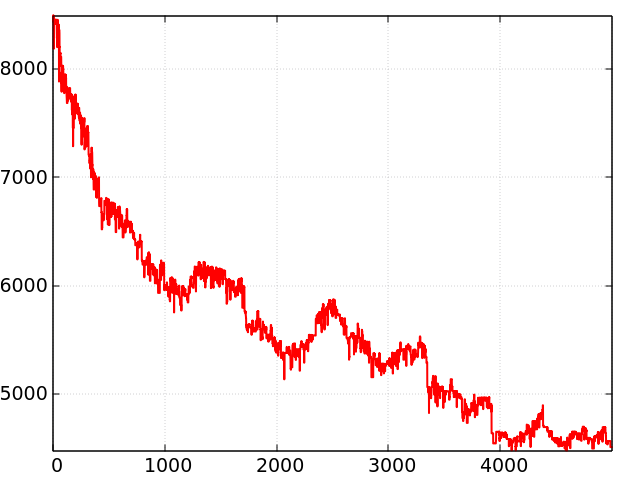
\includegraphics[width=\linewidth]{benchmark/convergence/sequentialConvergence.png}
	\subcaption{Sequential}\label{fig:sequential_convergence}
	\endminipage\hfill
	\minipage{0.32\textwidth}%
	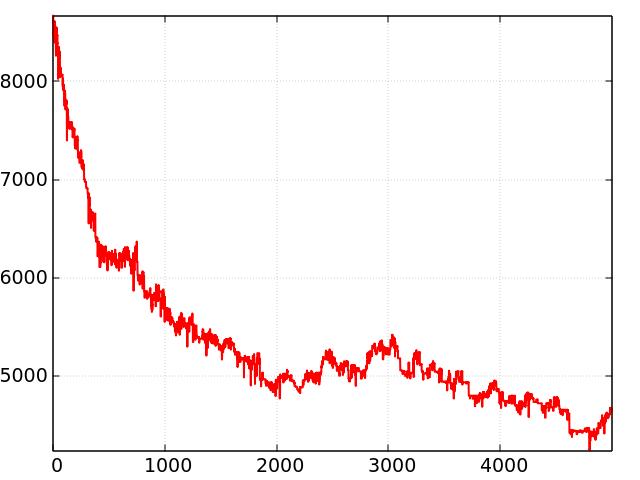
\includegraphics[width=\linewidth]{benchmark/convergence/standardConvergence.png}
	\subcaption{Standard thread}\label{fig:standard_convergence}
	\endminipage\hfill
	\minipage{0.32\textwidth}%
	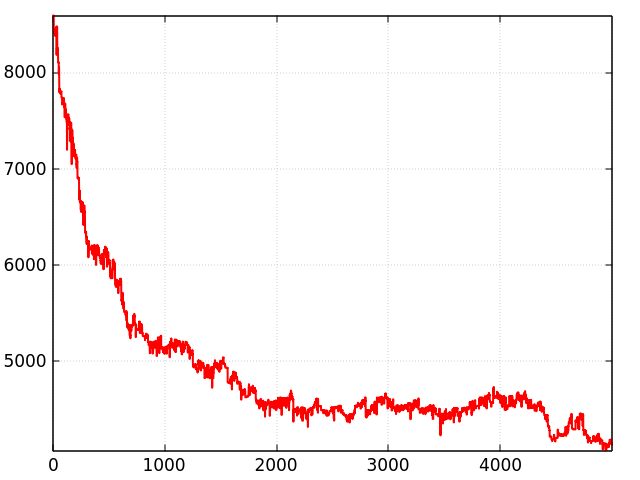
\includegraphics[width=\linewidth]{benchmark/convergence/fastflowConvergence.png}
	\subcaption{Fastflow}\label{fig:fastflow_convergence}
	\endminipage
	\caption{}\label{algorithmsConvergence}
\end{figure}

\subsection{Measures}
To compare and model the performance of a parallel program two performance indicators were used, \textit{speedup} and \textit{scalability}. For these metrics the speedup asymptote is given by $f(n) = n$.
\subsubsection{Speedup}
The \textit{speedup} is the ratio between the best known sequential execution time and the parallel execution time. It gives a measure of how good is our parallelization with respect to the best sequential computation. It is a function of \textit{n} the parallelism degree of the parallel execution.
\begin{equation}
speedup(n) = \frac{T_{seq}}{T_{par}(n)}
\end{equation} 
\vspace{-2em}
\subsubsection{Scalability}
The \textit{scalability} is the ratio between the parallel execution with degree equal to 1 and the parallel execution time with parallelism degree equal to \textit{n}. It measures how efficient is the parallel implementation in obtaining better performance on bigger parallelism degree.
\begin{equation}
scalab(n) = \frac{T_{par}(1)}{T_{par}(n)}
\end{equation}


\section{Parallel Architecture Design}
The program was designed to handle large graph as input (that implies large chromosome dimension). This was done by achieving data locality by modelling most of the application with \textit{Scanning} and \textit{Sorting} operation. As mentioned in \cite{algo-eng} RAM model fails to capture the running time for problems that have large data sets because of the I/O bottleneck. Indeed reading and writing data in sequential order or sorting the data to obtain requisite layout is less expansive than accessing data at random. This two operation, respectively \textit{std::for\_each} and \textit{std::sort}, were standardized and added to C++ until C++11 and are available inside the \textit{algorithm} header.

To exploit parallelism an initial analysis on the sequential version of the program was done. Each genetic operation was measured, by importing \textit{chrono} header library, to understand which part of the program needed to be parallelized and which not. This analysis was also useful to understand the proportion between the size of the graph and the time taken for each genetic algorithm operation. The following pie charts (figure \ref{fig:pie-chart-times}) were obtained by comparing each time spent by the operations that compose the algorithm, the number means the time taken in milliseconds to complete the operation. In both cases, the number of chromosomes taken into consideration was 2000 and the number of generation was 1.
\vspace{1.7em}

\begin{figure}[H]
	\centering
	\begin{minipage}[t]{0.55\linewidth}
		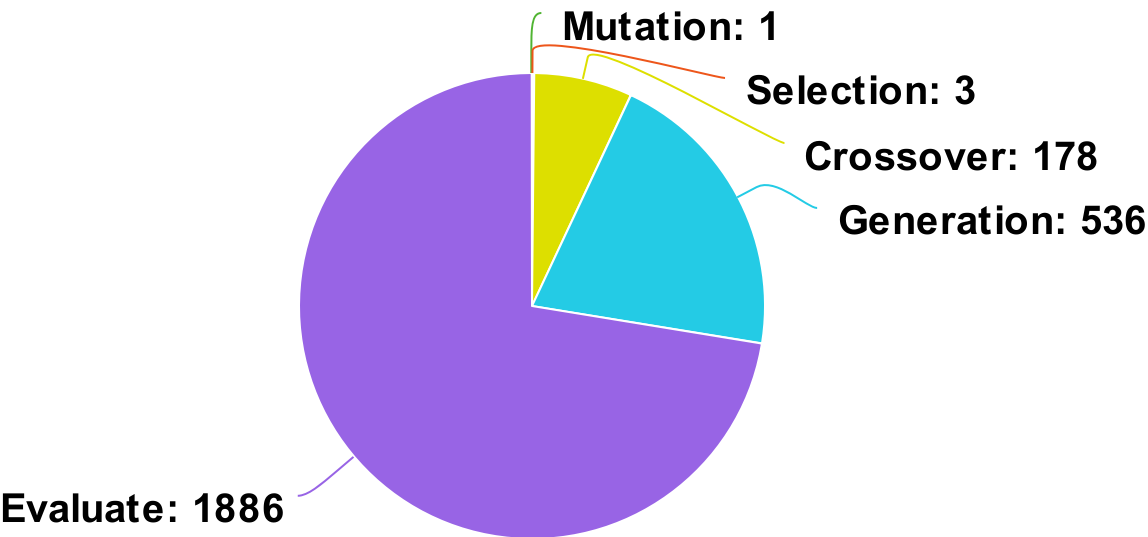
\includegraphics[width=\linewidth]{1000nodes6.png}
		\vspace{0.2em}
		\subcaption{1000 nodes} 
	\end{minipage}%
	\begin{minipage}[t]{0.57\linewidth}
		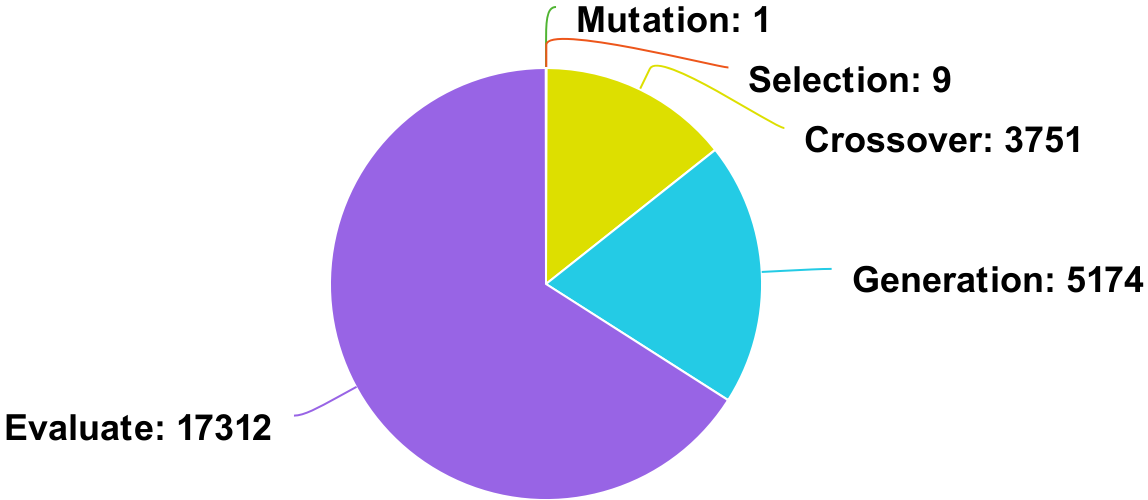
\includegraphics[width=\linewidth]{5000nodes5.png}
		\vspace{0.1em}
		\subcaption{5000 nodes}
	\end{minipage}
    \caption{}\label{fig:pie-chart-times}
\end{figure}

The first thing we noticed is that the most expansive operations are \textit{generation} (due to the random generation of the graph), \textit{evaluate} and \textit{crossover}.  Also, surprisingly, the selection phase that substitutes the old generation with the new one takes an insignificant amount of time. This is because all the index of the new population are sorted before the copy happens to exploit data locality and after the new generation is obtained (through \textit{Stochastic Universal Sampling} \cite{genetic-algorithm-tutorial}) the old generation is swapped with the new one, by moving the pointer, to avoid useless copy. 
\label{sez:architecture}

So, after the initial analysis I implemented the parallel versions by paying attention to the bottleneck created in \textit{evaluate}, \textit{generation} and \textit{crossover} phases. This was done by parallelizing the computation by splitting the works among multiple threads and then join the results obtained to proceed with the sequential computation of \textit{selection} and \textit{mutation} phases. Basically the high level structure of the program has the following operations form: 
\begin{figure}[H]
	\centering
	
\includegraphics[width=0.75\textwidth]{geneticAlgorithmStructure.png}
	%\caption{Genetic algorithm structure}
\end{figure}
 
\subsection{Standard thread implementation}
Since exception safety is an essential aspect of C++ code, I decided to use a modern C++ approach to spawn the workers to compute the genetic algorithm heavy operations in parallel. Indeed, spawning threads with the standard constructor offer by \textit{std::thread} object doesn't guarantee exception safety and an exception launched by a single thread can terminate the whole application. Also the destruction of the threads, when an exception arises, is not guaranteed and the program can have leak memory thread problems (also known as dangling thread problem).

So, I decided to use \textit{std::async} to spawn the threads with \textit{std::launch::async} to launch it asynchronously, this action produces a result stored in a \textit{std::future<T>} and the operation to be done by each thread is passed in-place as a lambda function with all the parameters needed for the computation as input. This approach guarantees that even if an exception is raised by a thread and its \textit{std::future} object is destroyed the destructor will wait for the thread to complete, so the memory thread leak problem is avoided. 

The model used is the fork/join one, this was chosen because each chunk computed by a worker has the same size and amount of work (computational time speaking) to be done. So a dynamic load balancing of the work between threads was not needed. Indeed the communication arrow between masters node (heavy operation of the genetic algorithm) and the workers are implemented as ``chunks'' (in the code a \textit{std::pair<start,end>}) of the main data structure that has the current population saved in it. The implementation has the skeleton reported in figure \ref{fig:standardStructure}: 
\vspace{1.5em}
\begin{figure}[h]
	\centering
	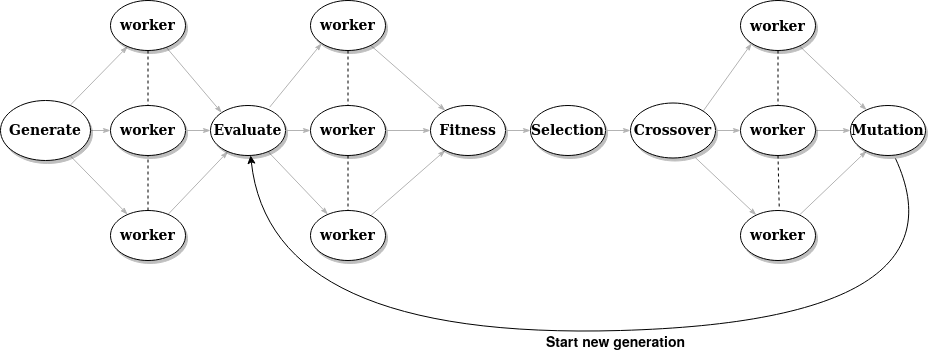
\includegraphics[width=1.1\textwidth]{standardMasterWorker.png}
	\vspace{0.15em}
	\caption{Standard C++ threads structure}
	\label{fig:standardStructure}
\end{figure}
\vspace{1em}

As we can see from figure \ref{fig:standardStructure} the first master worker spawning is done only at the beginning of the computation to speedup the random generation of the graph. This behaviour can be extended and modified, but basically the skeleton structure remains similar, to let the application parsing in parallel a file and create the graph. As mention above in \S \ref{sez:architecture} \textit{fitness} and \textit{selection} were designed as sequential computation because the time spent was too low (see \ref{fig:pie-chart-times} ) to obtain benefits exploiting parallelism.
 
\subsection{Fastflow implementation}
The version developed with Fastlow \cite{fastflow} was modelled using the information obtained from the analysis of the sequential algorithm (figure \ref{fig:pie-chart-times}). So, also in the Fastlow implementation the operations of \textit{generation}, \textit{evaluation} and \textit{crossover} were parallelized, moreover the communication between the emitters and collectors were chunks of indexes of chromosomes in the main data structure. The random generation of the graph was handled by creating a temporary farm with an emitter and a collector, but to save computational resources after the creation of the graph it is automatically deleted by the program. So the main skeleton of this version is composed by a pipeline composed by two farms (one for \textit{evalutation} and one for \textit{crossover}) and a sequential stage that computes the \textit{fitness} and \textit{selection} results. After creating the pipeline by injecting in the constructor the farms and the sequential node object the method \textit{wrap\_around()} is called to let the computation restarts from the initial emitter after all the current generation operations are done. 

\vspace{1.5em}
\begin{figure}[h]
	\centering
	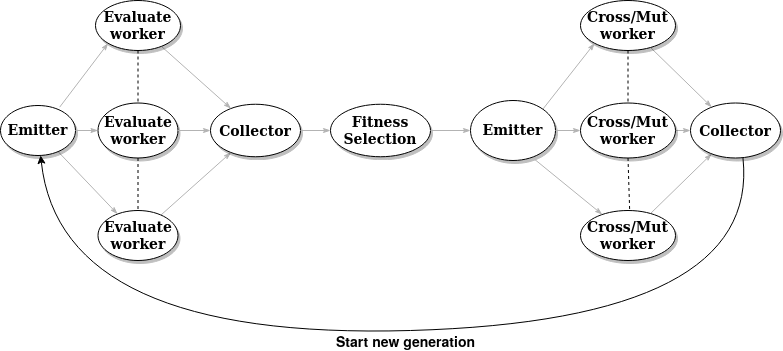
\includegraphics[width=1\textwidth]{fastflowMainStructure.png}
	\vspace{0.15em}
	\caption{Fastflow structure}
	\label{fig:fastflowStructure}
\end{figure}
\vspace{1em}

As we can see from figure \ref{fig:fastflowStructure} the sequential operations \textit{fitness} and \textit{selection} were merged in a single stage (node inside the pipeline) to save computational resources. Also every worker spawned by the second farm perform \textit{crossover} and immediately after that performs \textit{mutation} according to probabilities to optimize computational resources.

\section{Implementation details}
The project has three classes: \textit{fastflowTSP}, \textit{parallelTSP} and \textit{sequentialTSP}. If an object of \textit{Graph} type has been created and passed before in the constructor by calling the method \textit{Run} (and passing the parameters) the  algorithm starts. The user need to pass all the parameters by command line interface and then the program computes the three versions of the algorithm and for each of them the time spent is printed out. The only check is done on the number of workers by using \textit{std::thread::hardware\_concurrency()} method, if the user pass a number of workers that exceed the number returned by the method (so the supported thread of the machine are lower than the user specified threads), the number of thread is setted to the number returned by the method minus one. 
\section{Results}
Each version of the program was tested on the Xeon PHI machine, the tests were done with 10 generation and 20000 chromosomes and considering [500, 1000, 2000] nodes in the graph. As we can see from the curves, a good speedup is obtained with the first 50 threads because genetic algorithm are generally highly parallelizable algorithms. But as expected from the theory, after spawning more than 100 threads the overhead taken to set up and coordinate the computation is higher than the parallelism benefits obtained by adding threads. Surely with a bigger graph as input, the speedup curve would be increasing even with more than 100 threads. 

\subsection{Speedup curves}
\begin{figure}[H]
	\centering
\begin{minipage}[t]{0.50\linewidth}
	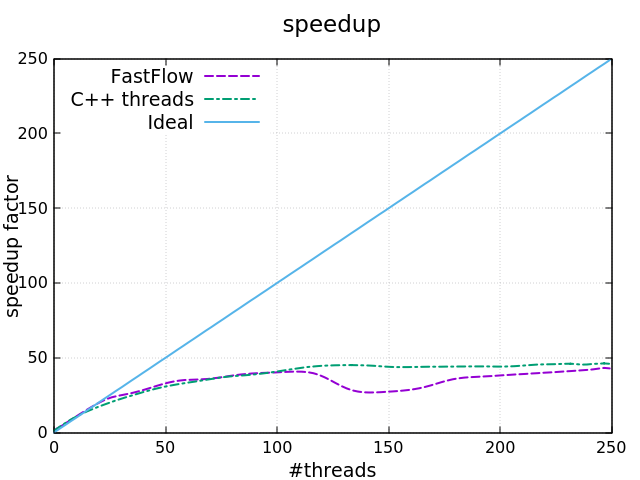
\includegraphics[width=\linewidth]{benchmark/curves/speedup_standard_2000_20000.png}
	\vspace{0.2em}
	%\subcaption{} 
\end{minipage}%
\begin{minipage}[t]{0.50\linewidth}
	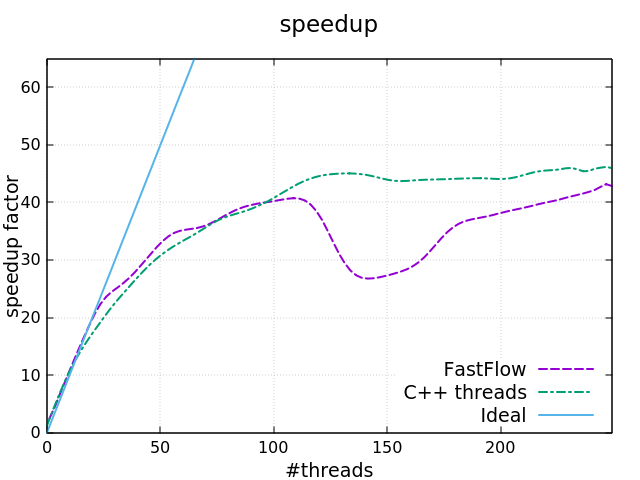
\includegraphics[width=\linewidth]{benchmark/curves/speedup_zoom_2000_20000.png}
	%\subcaption{}
\end{minipage}
\caption{Speedup 2000 nodes}\label{fig:speedup2000}
\end{figure}
\begin{figure}[H]
	\centering
	\begin{minipage}[t]{0.50\linewidth}
		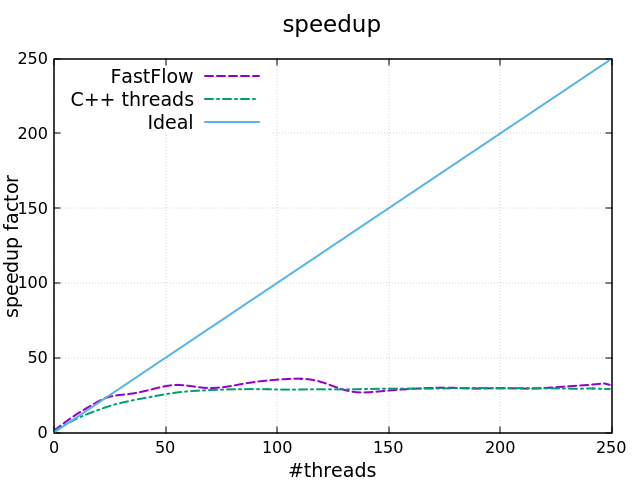
\includegraphics[width=\linewidth]{benchmark/curves/speedup_standard_1000_20000.png}
		\vspace{0.2em}
		%\subcaption{} 
	\end{minipage}%
	\begin{minipage}[t]{0.50\linewidth}
		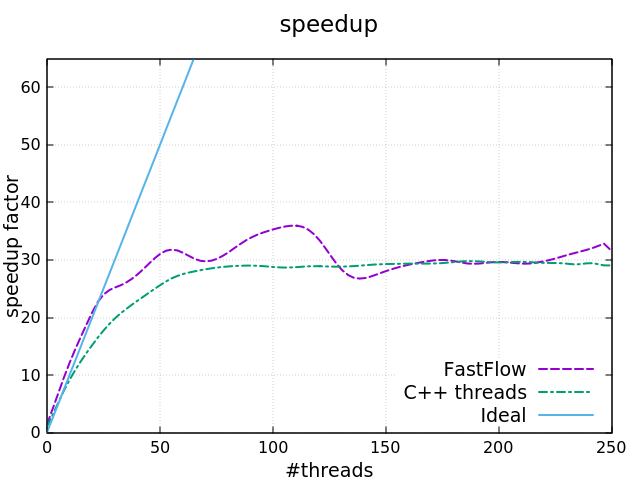
\includegraphics[width=\linewidth]{benchmark/curves/speedup_zoom_1000_20000.png}
		%\subcaption{}
	\end{minipage}
	\caption{Speedup 1000 nodes}\label{fig:speedup1000}
\end{figure}

\begin{figure}[H]
	\centering
	\begin{minipage}[t]{0.50\linewidth}
		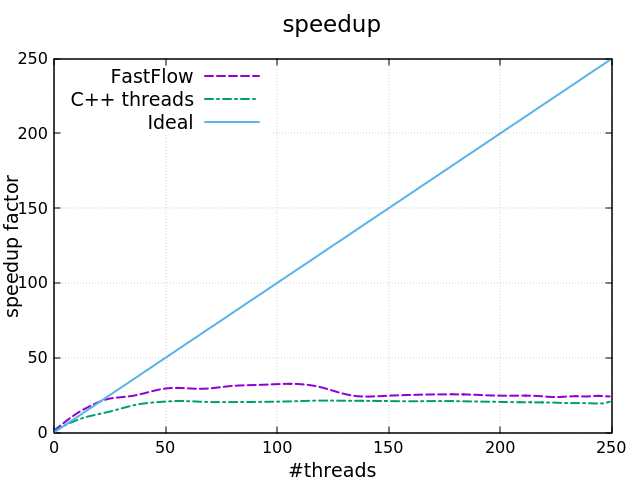
\includegraphics[width=\linewidth]{benchmark/curves/speedup_standard_500_20000.png}
		\vspace{0.2em}
		%\subcaption{} 
	\end{minipage}%
	\begin{minipage}[t]{0.50\linewidth}
		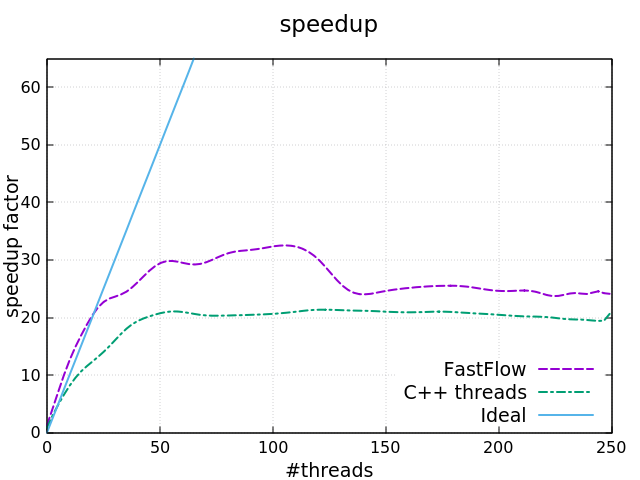
\includegraphics[width=\linewidth]{benchmark/curves/speedup_zoom_500_20000.png}
		%\subcaption{}
	\end{minipage}
	\caption{Speedup 500 nodes}\label{fig:speedup500}
\end{figure}

\subsection{Scalability curves}
\begin{figure}[H]
	\centering
\begin{minipage}[t]{0.50\linewidth}
	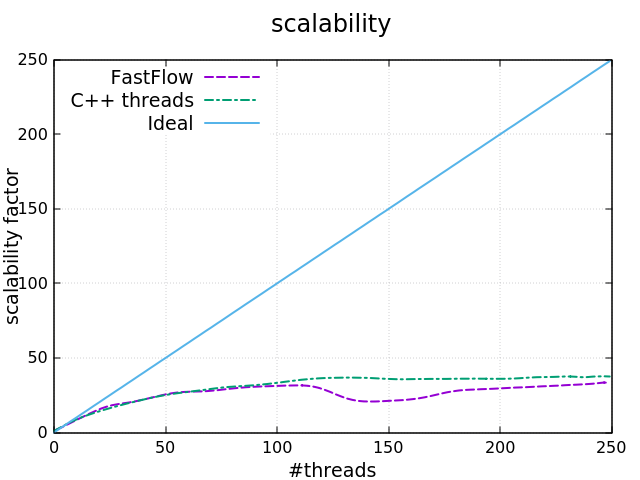
\includegraphics[width=\linewidth]{benchmark/curves/scalability_standard_2000_20000.png}
	\vspace{0.2em}
	%\subcaption{} 
\end{minipage}%
\begin{minipage}[t]{0.50\linewidth}
	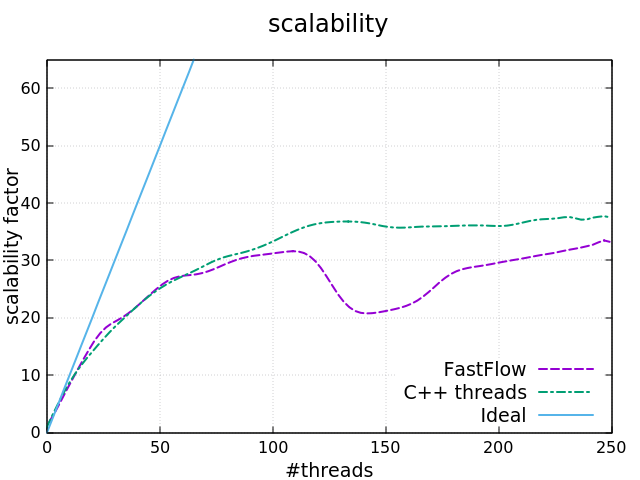
\includegraphics[width=\linewidth]{benchmark/curves/scalability_zoom_2000_20000.png}
	%\subcaption{}
\end{minipage}
\caption{Scalability 2000 nodes}\label{fig:scalability2000}
\end{figure}

\begin{figure}[H]
	\centering
	\begin{minipage}[t]{0.50\linewidth}
		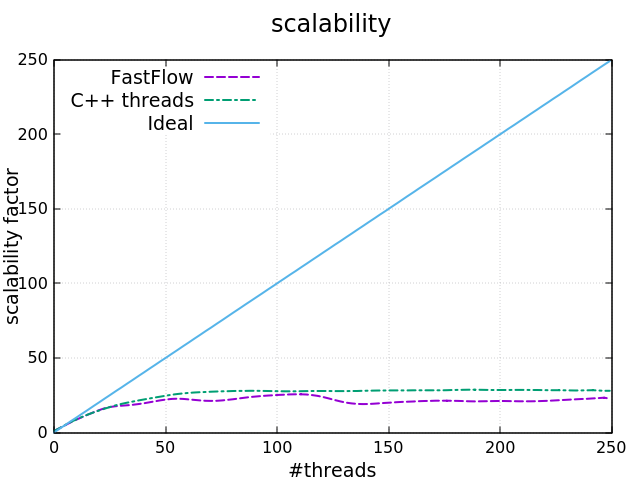
\includegraphics[width=\linewidth]{benchmark/curves/scalability_standard_1000_20000.png}
		\vspace{0.2em}
	%	\subcaption{} 
	\end{minipage}%
	\begin{minipage}[t]{0.50\linewidth}
		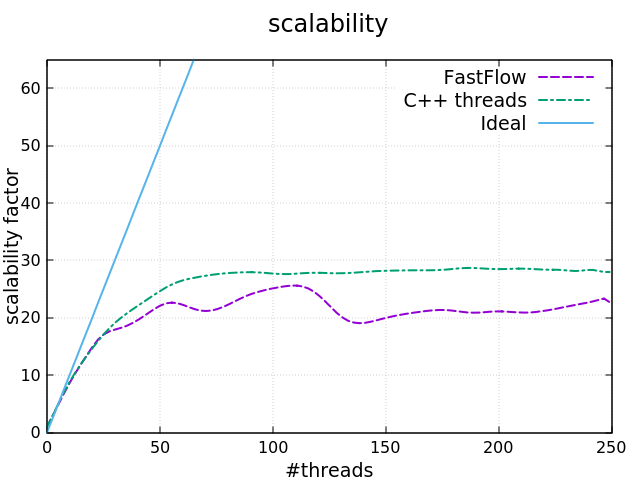
\includegraphics[width=\linewidth]{benchmark/curves/scalability_zoom_1000_20000.png}
	%	\subcaption{}
	\end{minipage}
	\caption{Scalability 1000 nodes}\label{fig:scalability2000}
\end{figure}

\begin{figure}[H]
	\centering
	\begin{minipage}[t]{0.50\linewidth}
		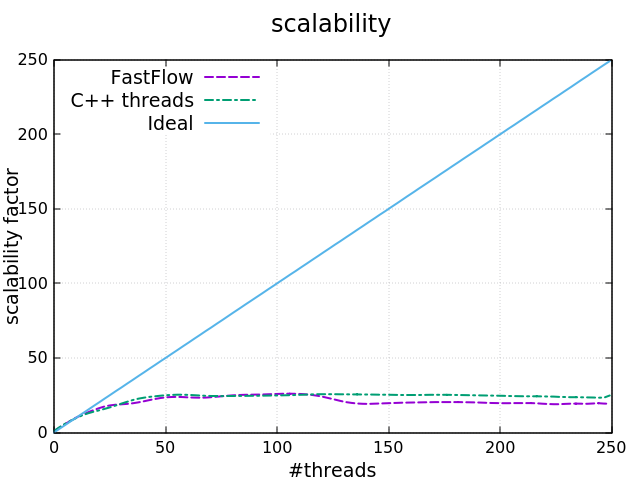
\includegraphics[width=\linewidth]{benchmark/curves/scalability_standard_500_20000.png}
		\vspace{0.2em}
	%	\subcaption{} 
	\end{minipage}%
	\begin{minipage}[t]{0.50\linewidth}
		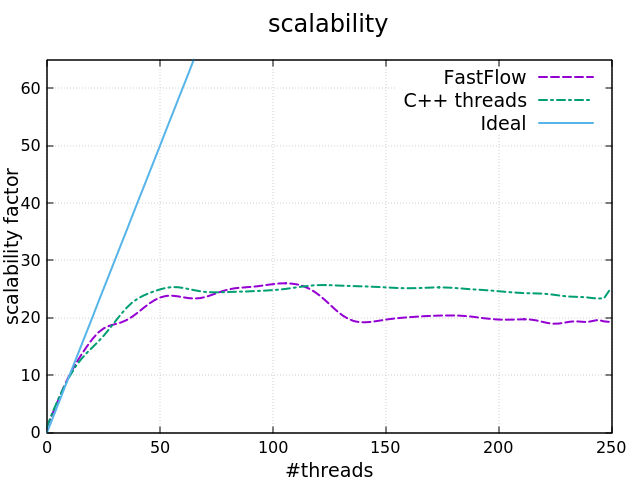
\includegraphics[width=\linewidth]{benchmark/curves/scalability_zoom_500_20000.png}
	%	\subcaption{}
	\end{minipage}
	\caption{Scalability 500 nodes}\label{fig:scalability2000}
\end{figure}
\section{Conclusion}
The project gave me the opportunity to apply the theory seen during the course to a real world problem. The initial design of the parallel architecture was strictly correlated to the results obtained from the analysis of the sequential program to find the application bottleneck. Also at the beginning it was challenging to deal with the parallel implementation of the algorithm with the standard C++ threads, the error generated by the parallel program were hard to find (and debugging) manually, but thanks to tools like Valgrind or ThreadSanitizer they were quite easy to found and fix. However, these errors made me understand the purpose of parallel skeleton framework like Fastflow that hide all the parallelism complexity to the programmer. 

\begin{thebibliography}{9}
	
	\bibitem{fastflow} 
	Marco Aldinucci, Marco Danelutto, Peter Kilpatrick, Massimo Torquati.
	\textit{Fastflow: high-level and efficient streaming on multi-core }. Programming Multi-core and Many-core Computing Systems
	\\\texttt{https://github.com/fastflow/fastflow}
	
	\bibitem{genetic-algorithm-tutorial} 
	Darrell Whitley.
	\textit{A genetic algorithm tutorial }. Kluwer Academic Publishers
	
	\bibitem{algo-eng} 
	Müller-Hannemann, Matthias, Schirra, Stefan.
	\textit{Algorithm Engineering}. Springer
	
	% \bibitem{PaperL-BFQS} 
	% Dong C. Liu and Jorge Nocedal.
	% \textit{On the limited memory BFGS method for large scale optimization}. Mathematical Programming 45 (1989), pp. 503-528.
	% \\\texttt{https://people.sc.fsu.edu/\textasciitilde inavon/5420a/liu89limited.pdf}
	
\end{thebibliography} 
\newpage
\input{sez/references.tex}
\end{document}
